%% Copyright (c) 2004  SciSoft.  All rights reserved.
%%
%% This file is part of CGAL (www.cgal.org); you may redistribute it under
%% the terms of the Q Public License version 1.0.
%% See the file LICENSE.QPL distributed with CGAL.
%%
%% Licensees holding a valid commercial license may use this file in
%% accordance with the commercial license agreement provided with the software.
%%
%% This file is provided AS IS with NO WARRANTY OF ANY KIND, INCLUDING THE
%% WARRANTY OF DESIGN, MERCHANTABILITY AND FITNESS FOR A PARTICULAR PURPOSE.
%%
%% 
%%
%% Author(s)     : Andreas.Fabri@geometryfactory.com, Fernando Cacciola <fernando_cacciola@hotmail.com>


Many geometric data structures can be interpreted as graphs, as they consist of
vertices, edges and faces. This is the case for the halfedge data structure,
for the polyhedron, for arrangements and for triangulations. With means of
duality one can also interpret faces as vertices and edges between adjacent
faces as edges of the dual graph. 


As the scope of \cgal\ is geometry and not graph algorithms, we
provide the necessary classes and functions that allow to use the
algorithms of the \ccAnchor{http://www.boost.org/libs/graph/doc/index.html}{Boost Graph Library ({\sc Bgl})} \cite{cgal:sll-bgl-02} for \cgal\ data structures.

\section{A Short Introduction to the Boost Graph Library}

The algorithms of the {\sc Bgl} operate on models of the various {\em graph concepts}. 
The {\em traits class} \ccc{boost::graph_traits} allows the algorithms to determine the types of vertices and edges. 
{\em Free functions} that operator on graphs allow the algorithms to obtain,
for example, the source vertex of an edge, or  all edges incident to a vertex. The algorithms 
use {\em property maps} to associate information to vertices and edges. 
The algorithms allow {\em visitors} to register callbacks that will be called
during the execution of the algorithms. Finally, the graph algorithms use
the {\em named parameter} mechanism, which allows to pass the  arguments in
arbitrary order.


\subsubsection*{Graph Concepts}

The {\sc Bgl} introduces several graph concepts, which have different sets of characteristics and requirements,
as for example whether one can enumerate all vertices or all edges, whether one only can get the outgoing 
edges of a vertex, or also the ingoing edges, or whether one can add and remove vertices and edges or not. 

Graph concepts in the {\sc Bgl} manual: \path|http://www.boost.org/libs/graph/doc/graph_concepts.html|


\subsubsection*{The Graph Traits Class}

The algorithms determine types with the help of the traits class
\ccAnchor{http://www.boost.org/libs/graph/doc/graph_traits.html}{\ccc{boost::graph_traits}}.  Such types are the \ccc{vertex_descriptor}
which is equivalent to a vertex handle in \cgal\ data structures, the
\ccc{vertex_iterator} which is similar to the vertex iterators in
\cgal\ data structures, and the \ccc{out_edge_iterator} which is
similar to edge circulators, which allow to enumerate the edges
incident to a vertex. The latter two are similar and not equivalent,
because their value type is a \ccc{vertex_descriptor}, whereas in
\cgal\ handles, iterators, and cicrulators all have the same value
type, namely the vertex type.  Given a graph type \ccc{G} the
declaration of a vertex descriptor looks as follows:
\ccc{boost::graph_traits<G>::vertex_descriptor vd;}.

\smallskip
The graph traits in the {\sc Bgl} manual: \path|http://www.boost.org/libs/graph/doc/graph_traits.html|

\subsubsection*{Free Functions for Exploring a Graph}

The algorithms obtain incidence information with the help of global
functions like \ccc{pair<vertex_iterator,vertex_iterator>
vertices(const Graph& g);} for getting an iterator range which allows
to enumerate all vertices, or \ccc{int num_vertices(const Graph&);} for getting the number of vertices of a graph, or
\ccc{vertex_descriptor source(edge_descriptor, const Graph&}, for
getting the source vertex of an edge. Note, that the
way we have written the types is a simplification, that is in reality
the signature of the first of the above functions is 
\ccc{pair<boost::graph_traits<Graph>::vertex_iterator,boost::graph_traits<Graph>::vertex_iterator> vertices(const Graph& g);}.

\smallskip
The free functions required for graph concepts: \path|http://www.boost.org/libs/graph/doc/graph_concepts.html|

\subsubsection*{Property Maps}

Another feature used heavily in the {\sc Bgl} is the {\em property map}
which is offered by the {Boost Property Map Library}.
Property maps are used to attach information to vertices and edges. It is again
a traits class and some free functions for obtaining the property map from
a graph, and  for getting and putting properties. 

The free functions are \ccc{get} and \ccc{put}.  The first one is overloaded.
One version allows to obtain a property map for a given property tag. For example
\ccc{m = get(g, boost::vertex_index)} gives us a property map that associates
an index in the range \ccc{[0, num_vertices(g))} to each vertex
descriptor of the graph.  The second version of the \ccc{get} function
allows to read it as follows for a vertex descriptor \ccc{vd}:
\ccc{int vdi = get(m, vd)}.  Just as \ccc{get} allows to read data,
\ccc{put} allows to write them.  For example, the Dijksta's shortest path algorithm writes
the predecessor of each vertex, as well as the distance to the source in such a 
property map.


The data themselves may be stored in the vertex or edge, or they may
be stored in an external data structure, or they may be computed on
the fly. This is an ``implementation detail'' of the particular property map.

\smallskip
Property maps in the Boost manuals: \path|http://www.boost.org/libs/property_map/property_map.html|

\subsubsection*{Visitors}

Visitors are ojects that provide functions that get called at
specified event points by the algorithm they visit.  The notion of
visitors is a design pattern, and also used in \cgal, e.g., the \ccc{Arr_observer<Arrangement>} 
in the arrangement package.  

The functions as well as the event points are library specific. Event
points in graph algorithms are, for example, when a vertex is traversed the first time, or when
all outgoing edges of a vertex are traversed.

\smallskip
Visitors in the {\sc Bgl} manual: \path|http://www.boost.org/libs/graph/doc/visitor_concepts.html|

\subsubsection{Named Parameters}

The algorithms of the {\sc Bgl} often have many parameters. Although the default
value is most often appropriate, one has to write them explicitly, if one only
wants to deviate from the default for the last one.  The solution to this problem
is to first write a tag and then the parameter, which for
Dijkstra's shortest path algorithm, might look as follows:


\begin{cprog} 
  std::vector<vertex_descriptor> p(num_vertices(g));
  std::vector<int> d(num_vertices(g));
  vertex_descriptor s = vertex(A, g);
  dijkstra_shortest_paths(g, s, predecessor_map(&p[0]).distance_map(&d[0]));
\end{cprog}

The named parameters in the example use the tags \ccc{predecessor_map} and \ccc{distance_map} and
they are concatenated with the dot operator.

\smallskip
Named parameters in the {\sc Bgl} manual: \path|http://www.boost.org/libs/graph/doc/bgl_named_params.html|

\section{Extensions of the BGL}

\cgal\ provides the partial specializations and free functions such that 
several data structures become model of some of the {\sc Bgl} graph concepts.
Furthermore, we define the new graph concept \ccc{HalfedgeGraph}, a traits class \ccc{halfedge_graph_traits},
and free functions for accessing opposite edges as well as the clockwise and
counterclockwise neighbor of an edge around a given vertex.

These extensions are used by the surface simplification algorithms which follow
the design of the {\sc Bgl} as sketched in the previous section.





\section{Header Files, Namespaces, and Naming Conventions}

As we interface two libraries we have to explain what resides in which namespace,
and what naming conventions we apply to what. 

Partial specializations of the \ccc{boost::graph_traits<Graph>} for the \cgal\ package
\ccc{Package} are in the namespace \ccc{boost} and in the headerfile \ccc{<CGAL/boost/graph/graph_traits_Package.h>}.

The \ccc{halfedge_graph_traits} class is in the namespace \ccc{CGAL},
but it is not capitalized as the \ccc{boost::graph_traits} is not.
The same holds for the types and enums for vertex and edge properties.





\section{Polyhedral Surfaces as Model of the Boost Graph Concept}

The class \ccc{Polyhedron_3} is model of the graph concept.  Furthermore
this chapter introduces a new graph concept, the \ccc{HalfedgeGraph}.

\subsection{Example: Minimum Spanning Tree of a Polyhedral Surface}

The example code computes the minimum spanning tree on a polyhedral surface.
More examples can be found in Chapter~\ref{chapter-meshsimplification} on surface mesh simplification.

\ccIncludeExampleCode{../examples/BGL/Polyhedron_3/kruskal.cpp}



\subsection{Example: Using Vertices, and Edges with an ID}

The following example program shows a call to the {\sc Bgl} 
Kruskal's minimum spanning tree algorithm accessing the id() 
field stored in a Polyhedron vertex.\\
The main function illustrates the access to the id() field.

\ccIncludeExampleCode{../examples/BGL/Polyhedron_3/kruskal_with_stored_id.cpp}



\section{Triangulations as Models of the Boost Graph Concept}

Triangulations have vertices and faces. Edges are pairs of a face and the
index of the edge.
Particular care has to be taken with the infinite vertex, and its incident
edges. One can either use a \ccc{boost::filtered_graph}, which makes the infinite edges
invisible, or one can have a property map that returns an infinite length
for these edges.


A classical example for an algorithm that is a combination of
computational geometry and graph theory is the {\em Euclidean Minimum
Spanning Tree} for a point set in the plane.  It can be computed by
running the minimum spanning tree algorithm on a Delaunay
triangulation of the point set.

\subsection{Example: Euclidean Minimum Spanning Tree}

In the following example we create a Delaunay triangulation and run Kruskal's minimum
spanning tree algorithm on it. Because the vertex handles of the triangulation are not indices
in an array, we have to provide a property map that maps vertex handles to
int's in the range \ccc{[0, t.number_of_vertices())}.

\ccIncludeExampleCode{../examples/BGL/Triangulation_2/emst.cpp}


\subsection{Example: Storing the Vertex ID in the Vertex}

The algorithms of the {\sc Bgl} extensively use of the indices of
vertices. In the previous example we stored the index in a \ccc{std::map}
and turned that map in a property map. This property map was then
passed as argument to the shortest path function.

If the user does not pass explicitly a property map, the graph algorithms
use the property map returned by the call \ccc{boost::get(boost::vertex_index,ft)}.
This property map assumes that the vertex has a 
member function \ccc{id()} that returns a reference to an int.
Therefore \cgal\ offers a class \ccc{Triangulation_vertex_base_with_id_2}.
It is in the users responsibility to set the indices properly.

The example further illustrates that the graph traits also works
for the Delaunay triangulation.

\ccIncludeExampleCode{../examples/BGL/Triangulation_2/dijkstra_with_internal_property.cpp}


\section{Arrangements as Models of the Boost Graph Concept}

For the arrangements \cgal\ offers the graph traits for the arrangement
itself as well as for its dual graph.


\subsection{Example for the Arrangement as Graph\label{arr_sssec:bgl_primal}}
%-------------------------------------------------

Arrangement instances are adapted to {\em boost} graphs by specializing the
\ccc{boost:graph_traits} template for \ccc{Arrangement_2} instances. The
graph-traits states the graph concepts that the arrangement class models
(see below) and defines the types required by these concepts.

In this specialization the \ccc{Arrangement_2} vertices correspond to the
graph vertices, where two vertices are adjacent if there is at least one
halfedge connecting them. More precisely, \ccc{Arrangement_2::Vertex_handle}
is the graph-vertex type, while \ccc{Arrangement_2::Halfedge_handle} is the
graph-edge type. As halfedges are directed, we consider the graph to be
directed as well. Moreover, as several interior-disjoint $x$-monotone curves
(say circular arcs) may share two common endpoints, inducing an arrangement
with two vertices that are connected with several edges, we allow parallel
edges in our {\em boost} graph.

Given an \ccc{Arrangement_2} instance, we can efficiently traverse its
vertices and halfedges. Thus, the arrangement graph is a model of the concepts
\ccc{VertexListGraph} and \ccc{EdgeListGraph} introduced by the \bgl.
At the same time, we use an iterator adapter of the circulator over the
halfedges incident to a vertex (\ccc{Halfedge_around_vertex_circulator} --- see
Section~\ref{arr_sssec:tr_vertex}), so it is possible to go over the ingoing
and outgoing edges of a vertex in linear time. Thus, our arrangement graph
is a model of the concept \ccc{BidirectionalGraph} (this concept refines
\ccc{IncidenceGraph}, which requires only the traversal of outgoing edges).

It is important to notice that the vertex descriptors we use are
\ccc{Vertex_handle} objects and {\em not} vertex indices. However, in order
to gain more efficiency in most {\sc Bgl} algorithm, it is better to have them
indexed $0, 1, \ldots, (n-1)$, where $n$ is the number of vertices. We
therefore introduce the \ccc{Arr_vertex_index_map<Arrangement>} class-template,
which maintains a mapping of vertex handles to indices, as required by the
\bgl. An instance of this class must be attached to a valid arrangement
vertex when it is created. It uses the notification mechanism (see
Section~\ref{arr_sec:notif}) to automatically maintain the mapping of vertices
to indices, even when new vertices are inserted into the arrangement or
existing vertices are removed.

In most algorithm provided by the \bgl, the output is given by
{\em property maps}, such that each map entry corresponds to a vertex.
For example, when we compute the shortest paths from a given source vertex
$s$ to all other vertices we can obtain a map of distances and a map of
predecessors --- namely for each $v$ vertex we have its distance from $s$
and a descriptor of the vertex that precedes $v$ in the shortest path from $s$.
If the vertex descriptors are simply indices, one can use vectors to
efficiently represent the property maps. As this is not the case with the
arrangement graph, we offer the \ccc{Arr_vertex_property_map<Arrangement,Type>}
template allows for an efficient mapping of \ccc{Vertex_handle} objects to
properties of type \ccc{Type}. Note however that unlike the
\ccc{Arr_vertex_index_map} class, the vertex property-map class is not
kept synchronized with the number of vertices in the arrangement, so it
should not be reused in calls to {\sc Bgl} functions in case the arrangement
is modified in between these calls.

\begin{figure}[t]
\begin{ccTexOnly}
  \begin{center}
  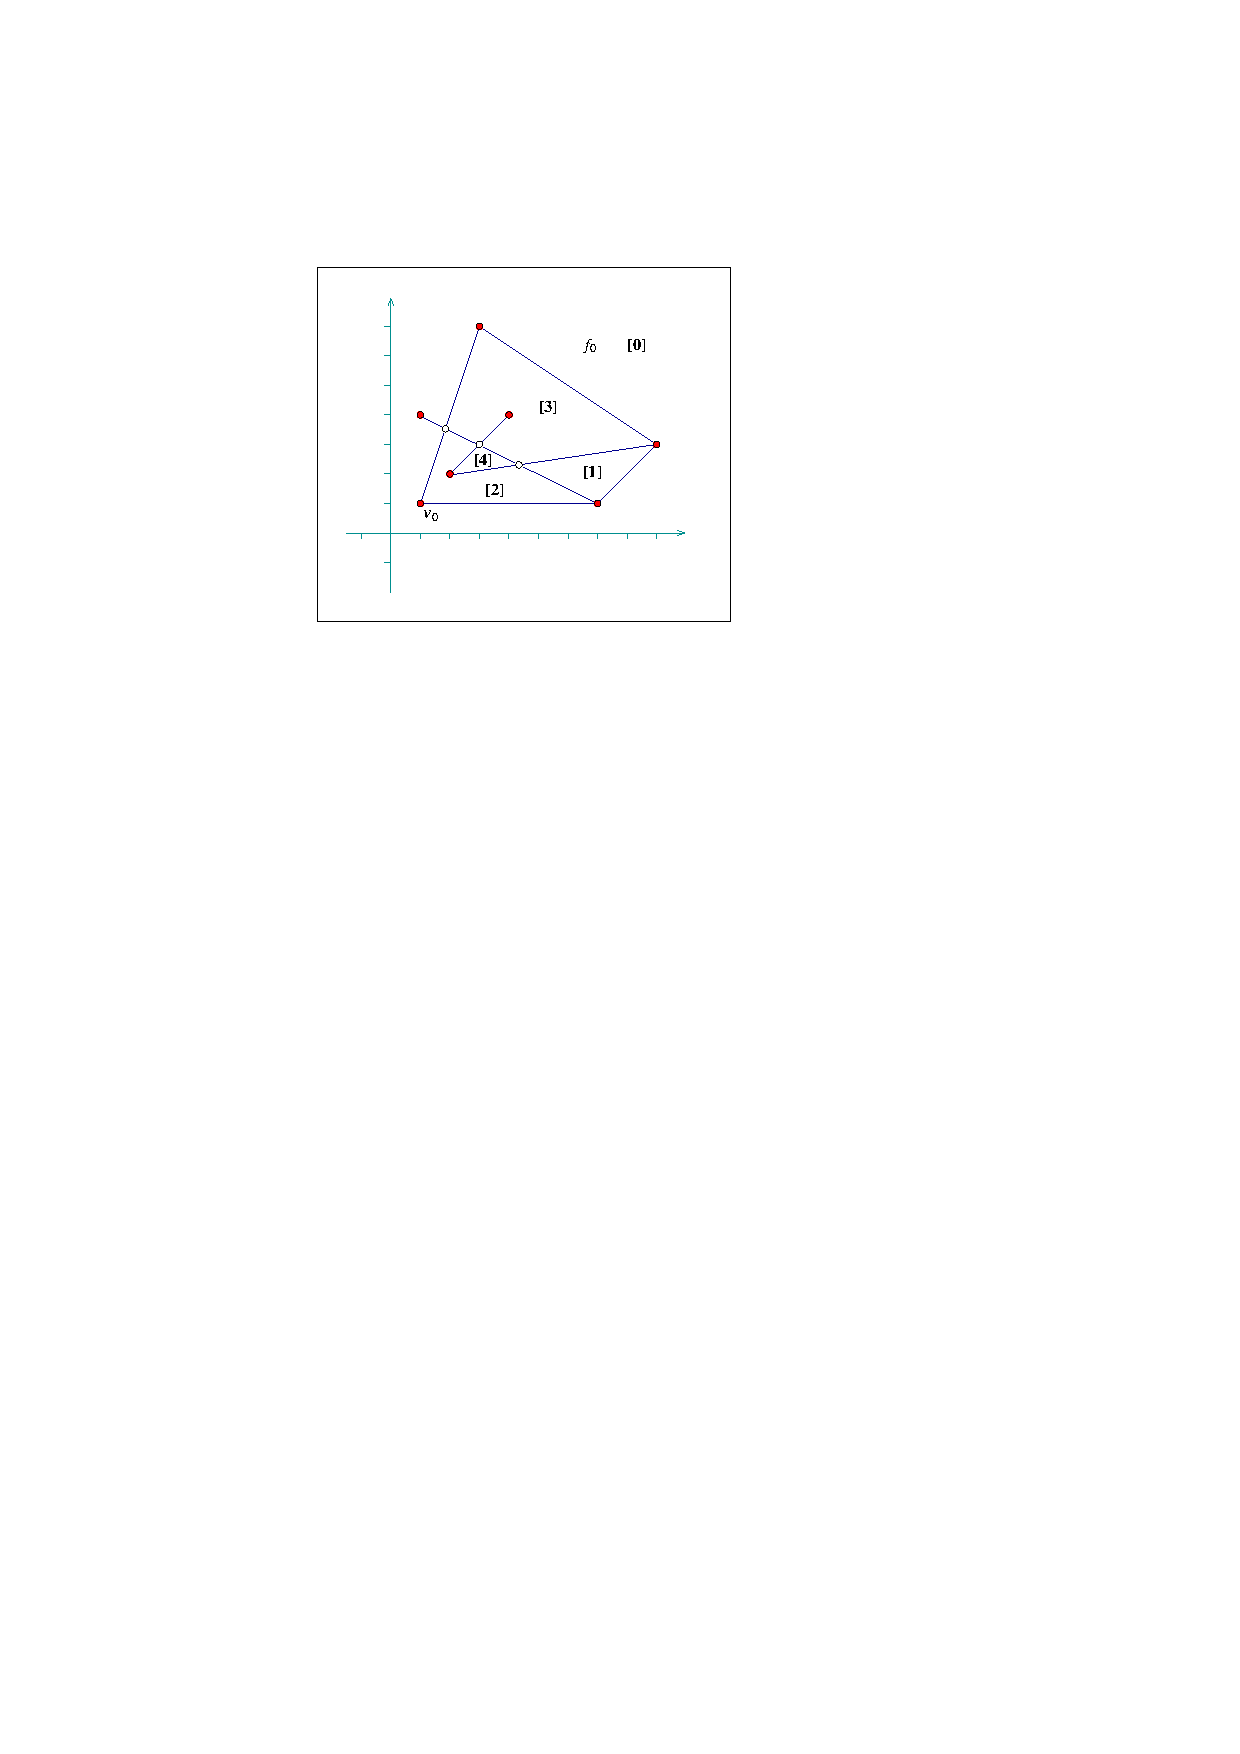
\includegraphics{BGL/fig/ex_bgl}
  \end{center}
\end{ccTexOnly}
\begin{ccHtmlOnly}
  <p><center>
  <img src="./fig/ex_bgl.gif" border=0 alt="Example BGL">
  </center>
\end{ccHtmlOnly}
\caption{An arrangement of 7 line segments, as constructed by
\ccc{ex_bgl_primal_adapter.cpp} and \ccc{ex_bgl_dual_adapter.cpp}.
The breadth-first visit times for the arrangement faces, starting
from the unbounded face $f_0$, are shown is brackets.}
\label{arr_fig:ex_bgl}
\end{figure}

In the following example we construct an arrangement of 7 line segments,
as shown in Figure~\ref{arr_fig:ex_bgl},
then use Dijkstra's shortest-paths algorithm from the {\sc Bgl} to compute
the graph distance of all vertices from the leftmost vertex in the
arrangement $v_0$. Note the usage of the \ccc{Arr_vertex_index_map} and
the \ccc{Arr_vertex_property_map} classes. The latter one, instantiated by
the type \ccc{double} is used to map vertices to their distances from $v_0$.

\ccIncludeExampleCode{../examples/BGL/Arrangement_2/primal.cpp}

\subsection{Example for the Dual of an Arrangement as Graph\label{arr_sssec:bgl_dual}}
%-----------------------------------------------

It is possible to give a dual graph representation for an arrangement instance,
such that each arrangement face corresponds to a graph vertex and two vertices
are adjacent iff the corresponding faces share a common edge on their
boundaries. This is done by specializing the
\ccc{boost:graph_traits} template for \ccc{Dual<Arrangement_2>} instances,
where \ccc{Dual<Arrangement_2>} is a template specialization that gives a
dual interpretation to an arrangement instance.

In dual representation, \ccc{Arrangement_2::Face_handle}
is the graph-vertex type, while \ccc{Arrangement_2::Halfedge_handle} is the
graph-edge type. We treat the graph edges as directed, such that a halfedge
\ccc{e} is directed from $f_1$, which is its incident face, to $f_2$, which
is the incident face of its twin halfedge. As two arrangement faces may
share more than a single edge on their boundary, we allow parallel
edges in our {\em boost} graph. As is the case in the primal graph, the dual
arrangement graph is also a model of the concepts \ccc{VertexListGraph},
\ccc{EdgeListGraph} and \ccc{BidirectionalGraph} (thus also of 
\ccc{IncidenceGraph}).

Since we use \ccc{Face_handle} objects as the vertex descriptors, we define
the \ccc{Arr_face_index_map<Arrangement>} class-template, which maintains an
efficient mapping of face handles to indices. We also provide the template
\ccc{Arr_face_property_map<Arrangement,Type>} for associating arbitrary
data with the arrangement faces.

In the following example we construct the same arrangement as in
example \ccc{ex_bgl_primal_adapter.cpp} (see Figure~\ref{arr_fig:ex_bgl}),
and perform breadth-first search on the graph faces, starting from the
unbounded face. We extend the \dcel\ faces
with an unsigned integer, marking the discover time of the face and use a
breadth-first-search visitor to obtain these times and update the faces
accordingly:

\ccIncludeExampleCode{../examples/BGL/Arrangement_2/dual.cpp}


% +------------------------------------------------------------------------+
%%RefPage: end of main body, begin of sfsooter
% EOF
% +------------------------------------------------------------------------+


